\documentclass[conference]{IEEEtran}
\IEEEoverridecommandlockouts
% The preceding line is only needed to identify funding in the first footnote. If that is unneeded, please comment it out.
\usepackage{cite}
\usepackage{amsmath,amssymb,amsfonts}
\usepackage{algorithmic}
\usepackage{graphicx}
\usepackage{textcomp}
\usepackage{xcolor}

\def\BibTeX{{\rm B\kern-.05em{\sc i\kern-.025em b}\kern-.08em
    T\kern-.1667em\lower.7ex\hbox{E}\kern-.125emX}}
\begin{document}

\title{City of Austin Car Crashes}

\author{\IEEEauthorblockN{Luca Comba}
\IEEEauthorblockA{\textit{University of St Thomas} \\
St Paul, MN \\
comb6457@stthomas.edu}
\and
\IEEEauthorblockN{Hung Tran}
\IEEEauthorblockA{\textit{University of St Thomas} \\
St Paul, MN \\
@stthomas.edu}
\and
\IEEEauthorblockN{Steven Tran}
\IEEEauthorblockA{\textit{University of St Thomas} \\
St Paul, MN \\
@stthomas.edu}
}

\maketitle

\begin{abstract}
After gathering the City of Austin's data set with over 216,000 reported car crashes from 2010, we were able to examine the relationship between various crash factors and their associated comprehensive costs using multiple machine learning approaches. Seven regression models, including Linear Regression, Ridge, LASSO, Decision Trees, Random Forest, Support Vector Regression, and K-Nearest Neighbors, were implemented to predict the estimated total comprehensive cost of accidents. 

The data set, part of Austin's Vision Zero initiative, includes features such as crash severity, vehicle types involved, and environmental conditions. Our analysis demonstrates that simpler regression models achieved the highest prediction accuracy with an R-squared value close to 1, providing valuable insights for urban planning and traffic safety improvements. The findings of this paper could contribute to understanding the economic impact of traffic accidents and can inform evidence-based policy decisions for accident prevention in urban environments.
\end{abstract}

\begin{IEEEkeywords}
austin, texas, car, crash, accidents, machine learning, linear regression, ridge, lasso, svr
\end{IEEEkeywords}

\section{Introduction}
The United States of America is heavily dependent on car transportation. Past data showed that "US cities in 1990 have levels of per capita auto use that are some two times higher than Australian cities \cite{b1}." Driving can be a dangerous and life-threatening action. A study conducted by the All India Institute of Medical Sciences (AIIMS) has shown that "the proportion of fatal accidents in total road accidents has consistently increased since 2002 from 18.1\% to 24.4\% in 2011\cite{b2}."

With the advent of new technologies and the publication of new open source machine learning libraries such as Scikit-learn which is "a machine learning package in the Python programming language that is widely used in data science \cite{b3}", it has been easier to analyze publicly available data set.

The City of Austin, Texas (U.S.A.), in the last few years, has started a new city project to better understand and prevent car accidents. The Austin Transportation program has worked on the "Vision Zero" project to create a transportation network that protects human life. The intent of the project is to design a city network that focuses on safety for all of its citizens\cite{b5}. Our research project will heavily rely on the Vision Zero project and on its powerful data set that will be discussed in the next section. The research effort aims at empowering the data collected by the City of Austin, and better understand the current situation of car accidents as well as the Estimated Total Comprehensive Cost of a car accident.

\subsection{The Austin Crash Report}
The Austin Crash Report Data Set\cite{b6} includes records of traffic accidents in the city of Austin, Texas, from 2010 to today, with 216,088 instances and 45 features, including both numerical and categorical data. The data set is managed by the Texas Department of Transportation, and utilized by Crash Record Information System database, which is populated by reports submitted by Texas Peace Officers throughout the state, including Austin Police Department.

The original data is composed by 45 features. In general terms, the data set had information about aspects such as location (latitude / longitude), crash timestamp, speed limit, severity (0-5), injury and death counts, type of vehicle involved, and the estimated total comprehensive cost. Many of these features will be used for training the machine learning models.

\subsection{Estimated Total Comprehensive Cost}
The Austin's Vision Zero initiative quantifies the impact of traffic crashes using comprehensive costs, which integrate both economic factors such as medical expenses, lost wages. The comprehensive cost also monetized quality of life impacts based on national guidelines. This total societal cost per crash is derived from National Safety Council and Federal Highway Administration methodologies \cite{b7}.

These comprehensive crash costs are a critical tool for Austin's transportation planning, enabling a data-driven approach to understanding and mitigating traffic-related harm. In our research, we focused on predicting the Estimated Total Comprehensive Cost as a key metric. This predicted value allows us to analyze its relationship with various factors, such as posted speed limits and vehicle types involved, to inform future safety interventions and policy decisions.

\begin{figure}
    \centering
    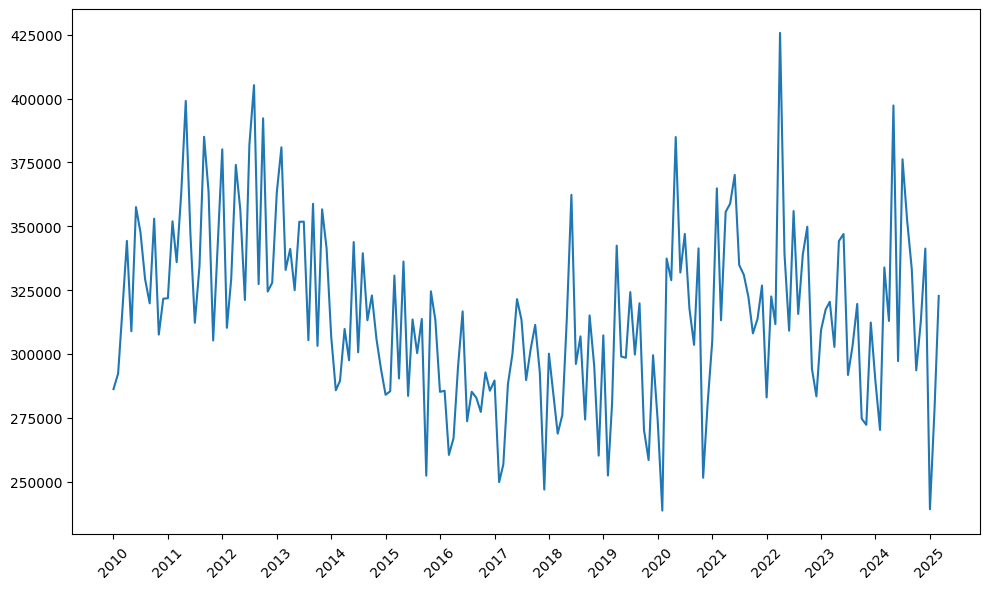
\includegraphics[width=1\linewidth]{total_cost_by_month.png}
    \caption{Total Comprehensive Cost by month}
    \label{fig:enter-label}
\end{figure}

\subsection{Data Exploration}
An exploratory data analysis was conducted on the The Austin Crash Report Data Set previously introduced. After an initial examination of the data types and a confirmation of no missing values a basic descriptive statistics such as mean, median, and standard deviation were computed for key cost-related variables, specifically on the estimated\_total\_comprehensive\_cost, to understand their central tendencies and spread. It was discovered that the total\_comprehensive\_cost mean was of 307,980\$.

It was then discovered that most of the crashes resulted in a non-significant severity, and in a non fatal crash. It is calculated that the data set has a 0.65\% death rate of all accidents (Fig. 3). 

The distribution of the speed limits contained in the data set shows a normal distribution, centered around 45 miles per hour (Fig. 4).

\begin{figure}
    \centering
    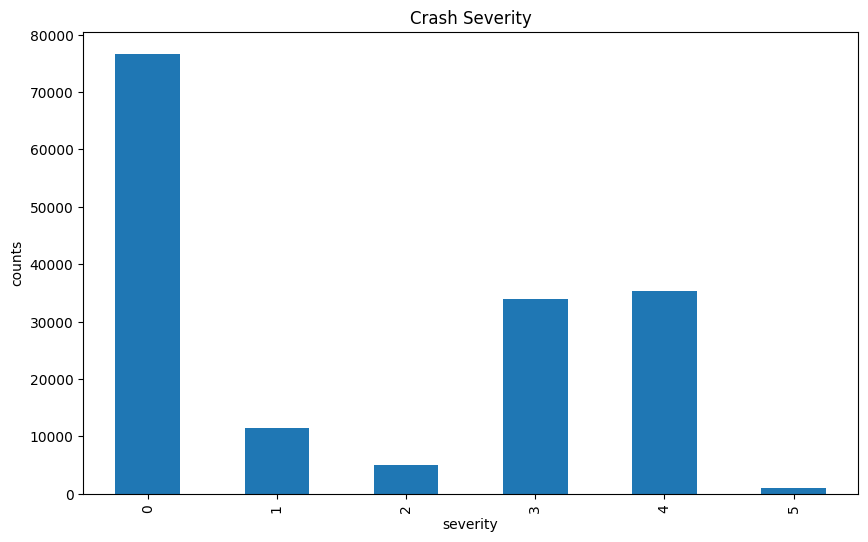
\includegraphics[width=1\linewidth]{final_images/crash_severity.png}
    \caption{Crash Severity counts}
    \label{fig:enter-label}
\end{figure}

\begin{figure}
    \centering
    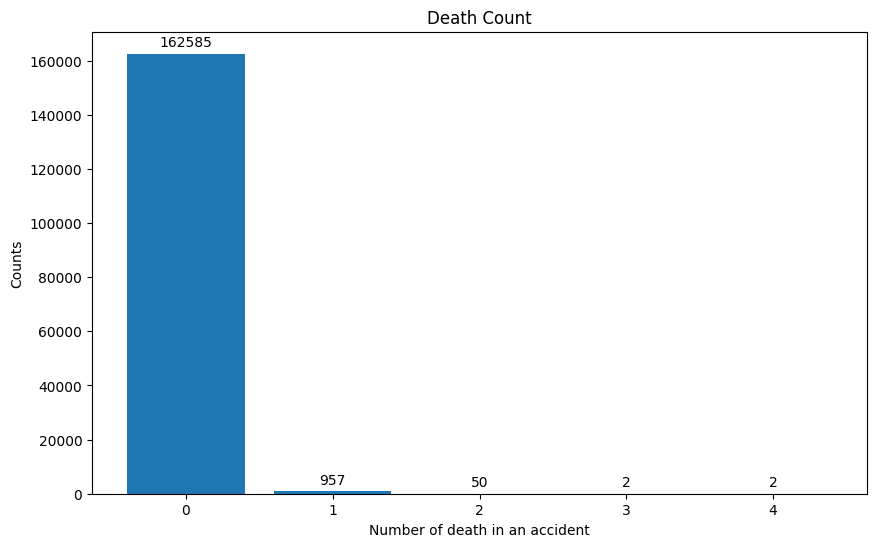
\includegraphics[width=1\linewidth]{final_images/death_count.png}
    \caption{Crash severity counts. From the least severe (0) to the most severe crashes (5)}
    \label{fig:enter-label}
\end{figure}

\begin{figure}
    \centering
    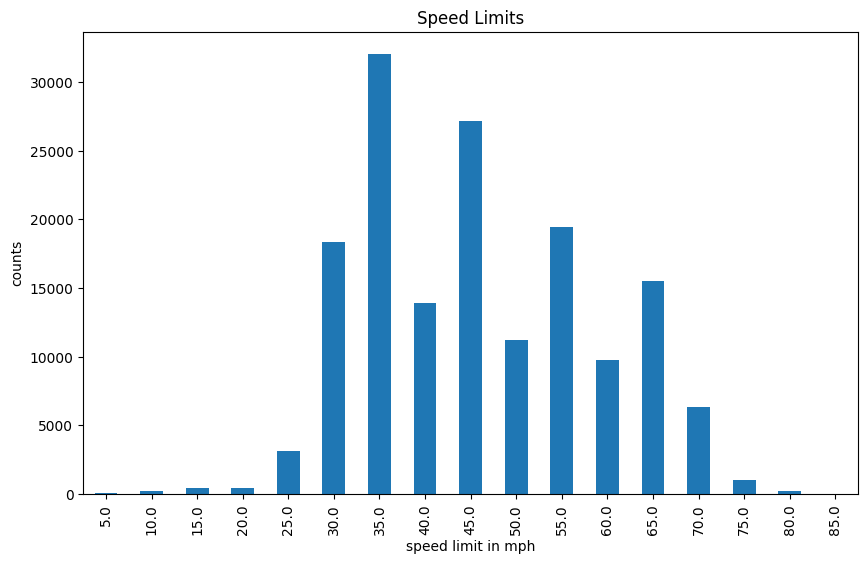
\includegraphics[width=1\linewidth]{final_images/speed_limits.png}
    \caption{Speed limits represented in the data set in mph}
    \label{fig:enter-label}
\end{figure}

\section{Data Cleansing}
The data set utilized underwent a comprehensive, multistage cleaning process to ensure data quality and suitability for subsequent analysis.

The initial phase of the data cleaning, focused on several data transformations. First, records flagged as temporary or deleted were removed from the original data set. Following this, a significant number of columns were determined to be redundant or not conducive to the modeling process and were consequently dropped. This included various identifier columns such as 'ID', 'Crash ID', and 'case\_id'. Columns containing repetitive address details such as 'rpt\_block\_num', 'rpt\_street\_name', 'rpt\_street\_sfx'. A 'point' column derived from geographic coordinates, and the 'Reported street prefix' were also removed. Additionally, columns pertaining to road type like the 'private\_dr\_fl', 'onsys\_fl' columns were excluded as initial exploration revealed no instances of accidents on private roads. After deriving a new 'Crash timestamp (US/Central)' from the original column 'Crash timestamp', the latter was dropped. The 'estimated\_maximum\_comprehensive\_cost' was removed from the feature set as it would be a repetition of the predictive variable which we have set to the Estimated Total Comprehensive Cost.

To have consistent data types and appropriate formatting we applied some other data transformation. Column naming conventions were standardized by converting all names to lowercase and replacing spaces with underscores ('Primary address' became 'primary\_address'). The 'Crash timestamp (US/Central)' column was converted into a datetime object to facilitate time-based feature engineering. Further, several columns received more descriptive names; for example, 'crash\_fatal\_fl' was changed to 'fatal\_crash', 'crash\_speed\_limit' to 'speed\_limit', and 'crash\_sev\_id' to 'crash\_severity'.

Additional value corrections and transformations were needed for the easy of use by the future machine learning models. For the 'speed\_limit' feature, values of -1 and 0, likely representing missing or erroneous data, were replaced with NaN and subsequently removed. The remaining 'speed\_limit' values were then binned by rounding them down to the nearest multiple of 5. This was done for helping with a data visualization effort. 

The 'crash\_severity' column, which initially had a nominal encoding, was remapped to an ordinal scale (0=NOT INJURED, 1=UNKNOWN, 2=POSSIBLE INJURY, 3=NON-INCAPACITATING INJURY, 4=INCAPACITATING INJURY, 5=KILLED) to represent it from the lowest to the highest value. These remapped categories were then one-hot encoded to create individual binary features for each severity level. 

The 'units\_involved' column, a textual description of vehicles in an accident, was also extensively processed. Combinations of units appearing infrequently, occurences of less than 1000 were filtered out. Unique vehicle types were then parsed from these strings, and new binary indicator columns were generated for each type, such as 'unit\_involved\_bicycle'. The original 'units\_involved' column was then discarded. 

Furthermore, the 'timestamp\_us\_central' feature was leveraged to engineer new time-related attributes, including 'hour', 'day\_of\_week', 'month', 'year', 'day\_of\_month', and a binary 'weekend' indicator. To capture the cyclical nature of time, sine and cosine transformations were applied to the 'hour' and 'month' features, creating 'hour\_sin', 'hour\_cos', 'month\_sin', and 'month\_cos'. 

Finally, any remaining rows containing NaN values after these steps were removed to ensure a complete data set.

Our final machine learning models did not utilized other columns that were kept after the cleaning of the data set. The unutilized columns were: 'primary\_address', 'secondary\_address', 'timestamp\_us\_central', 'latitude', and 'longitude'. This decision was made due to their data types or their deemed relevance for the specific modeling approach chosen. Although geo-spatial features like latitude and longitude could have been used for creating location clusters, they were excluded in this analytical iteration for the need of simpler models. 

Lastly, for modeling purposes, the target variable, 'estimated\_total\_comprehensive\_cost', was scaled by a factor of 100,000. The previously described cleaning and preparation stages resulted in a refined dataset optimized for the subsequent feature selection and model development processes.

\section{Feature Selection}
Given our dataset has 45 features, some might be redundant and irrelevant, potentially causing a longer computation time and reducing the efficiency of the models. To make sure our model concentrates on only useful independent variables, we select backward elimination to remove nonsignificant features that have a p-value under 0.05, avoid overfitting, and increase the overall performance of all models. 

\begin{center}
    {Backward Elimination}
\end{center}
\subsection*{Overview}
This method will start with the full 47 features in the original data set and remove the higher p-value feature in each iteration until all remaining features are statistically significant.  By following this approach, our dataset will left with only relevant features to use for predictive purpose. 

\subsection*{Result}
Here is a list of 19 features that have been eliminated: 

\begin{itemize}
    \item {month}
    \item {construction\_zone}
    \item {unit\_involved\_large\_passenger\_vehicle}
    \item {month\_sin}
    \item {day\_of\_month}
    \item {unit\_involved\_pedestrian}
    \item {day\_of\_week}
    \item {severity\_possible\_injury}
    \item {severity\_incapacitating\_injury}
    \item {severity\_non\_incapacitating\_injury}
    \item {law\_enforcement\_fatality\_count}
    \item {unit\_involved\_bicycle}
    \item {year}
    \item {death\_cnt}
    \item {tot\_injry\_cnt}
    \item {unit\_involved\_passenger\_car}
    \item {month\_cos}
    \item {hour\_sin}
    \item {unit\_involved\_other\_unknown}
\end{itemize}

\section{Feature Scaling}
\subsection{Target Variables}
As our input variables are mostly in the range 1 to 10, we decided to divide our target variables (Estimated Total Comprehensive Cost) by 100,000 to ensure numerical stability and potentially help improve computation efficiency. 

\subsection{Independent Variables}
We will apply Standardization to center the numerical data around the mean of 0 and the standard deviation of 1. Boolean columns will remain unchanged. 

\section{Methodology}
To predict the estimated total comprehensive cost, we will use 7 different machine learning models (listed below). In order to improve consistency and code organization, we will also leverage a pipeline function in sklearn. It allows preprocessor settings, which will be helpful in our later step of hyperparameter tuning. 

\subsection{Linear Regression}
This method will capture a linear relationship, and by comparing the coefficients, we can evaluate how each feature impacts the target variables and by how much. 

\subsection{Ridge Regression}
This method will work well with a multiple-feature dataset and can penalize non-significant ones, closing the gap between training and testing errors, leading to overfitting prevention. 

\subsection{LASSO Regression}
This method will apply L1 regularization, automatically do feature selection by shrinking the coefficients of non-significant features to zero,  helping to reduce overfitting. 

\subsection{Decision Tree Regression}
This method will capture non-linear relationships and won't be impacted by outliers while predicting the cost. 

\subsection{Random Forest Regression}
This method combines multiple decision trees to enhance the models' accuracy.  

\subsection{Support Vector Regressor (SVR) Regression}
This method will use kernels to handle non-linear data, transform our dataset to high-dimensional spaces, and then choose the best hyperplane to reduce prediction errors. 

\subsection{K-Nearest Neighbors Regressor (KNN) Regression}
This method will apply a non-parametric approach to capture complex relationships, and then use only local variations to predict the cost. 


\section{Results}
This document is a model and instructions for \LaTeX.
Please observe the conference page limits. 

\section{Conclusion}
This document is a model and instructions for \LaTeX.
Please observe the conference page limits. 

\begin{thebibliography}{00}
\bibitem{b1}J. R. Kenworthy and F. B. Laube, “Automobile dependence in cities: An international comparison of urban transport and land use patterns with implications for sustainability,” Environmental Impact Assessment Review, vol. 16, no. 4–6, pp. 279–308, Jul. 1996, doi: https://doi.org/10.1016/s0195-9255(96)00023-6.
\bibitem{b2}M. Ruikar, “National statistics of road traffic accidents in India,” Journal of Orthopedics, Traumatology and Rehabilitation, vol. 6, no. 1, p. 1, 2013, doi: https://doi.org/10.4103/0975-7341.118718.
\bibitem{b3}J. Hao, “Machine Learning Made Easy: A Review of Scikit-learn Package in Python Programming Language,” Journal of Educational and Behavioral Statistics, vol. 44, no. 3, p. 107699861983224, Feb. 2019, doi: https://doi.org/10.3102/1076998619832248.
\bibitem{b4}“Data.gov,” Data.gov, 2024. https://catalog.data.gov/dataset/vision-zero-crash-report-data
\bibitem{b5}“Vision Zero Viewer” visionzero.austin.gov. https://visionzero.austin.gov/viewer/
\bibitem{b6}City of Austin Texas, “Austin Crash Report Data - Crash Level Records,” Austintexas.gov, Jul. 30, 2019. https://data.austintexas.gov/Transportation-and-Mobility/Austin-Crash-Report-Data-Crash-Level-Records/y2wy-tgr5/about\_data
‌\bibitem{b7}“Comprehensive Crash Costs | AustinTexas.gov,” Austintexas.gov, 2018. https://www.austintexas.gov/crashcosts

\end{thebibliography}

\end{document}
